\documentclass[a4paper,11pt]{article}
\usepackage[margin=23mm,headheight=15pt]{geometry}
\usepackage{amsmath,amssymb,booktabs,tabularx,array,enumitem,xcolor,hyperref,fancyhdr,pgfplots,microtype}
\usepackage[section]{placeins}
\AddToHook{cmd/subsection/before}{\FloatBarrier}
\pgfplotsset{compat=1.18}
\definecolor{ink}{HTML}{20384B}
\definecolor{sppcolor}{HTML}{0072B2}
\definecolor{bopcolor}{HTML}{D55E00}
\hypersetup{colorlinks=true,linkcolor=ink,urlcolor=ink,citecolor=ink,pdftitle={Reproduction and Analysis of the Signature Path Prefetcher},pdfauthor={}}
\setlist{nosep,leftmargin=1.7em}
\renewcommand{\arraystretch}{1.18}
\setlength{\parskip}{4pt}
\setlength{\emergencystretch}{2em}
\setlength{\textfloatsep}{10pt plus 2pt minus 2pt}
\setlength{\intextsep}{10pt plus 2pt minus 2pt}
\setlength{\floatsep}{10pt plus 2pt minus 2pt}
\setlength{\abovecaptionskip}{6pt}
\setlength{\belowcaptionskip}{6pt}
\renewcommand{\topfraction}{0.85}
\renewcommand{\bottomfraction}{0.75}
\renewcommand{\textfraction}{0.10}
\raggedbottom
\pagestyle{fancy}
\fancyhf{}
\fancyhead[L]{\small Signature Path Prefetcher}
\fancyhead[R]{\small Technical Report}
\fancyfoot[C]{\thepage}
\newcolumntype{Y}{>{\raggedright\arraybackslash}X}
\newcommand{\code}[1]{\texttt{#1}}
\begin{document}

\begin{center}
{\LARGE\bfseries Reproduction and Analysis of the Signature Path Prefetcher}\par
\vspace{9pt}
{\large Path Confidence, Lookahead, and Workload Performance}\par
\vspace{10pt}
Student: \par
Date: October 7, 2026\par
\end{center}

\begin{abstract}
Hardware data prefetching can reduce memory stalls by bringing data into the cache before it is needed. Its effectiveness depends on timely predictions and the resources consumed by additional requests. The Signature Path Prefetcher (SPP) represents recent address deltas with a signature, learns possible continuations, and uses path confidence to control multistep prediction. This report explains the mechanism and evaluates SPP in ChampSim, using no data prefetching and the Best-Offset Prefetcher (BOP) as baselines.

The reproduction uses eight SPEC CPU2006 applications with 200 million warmup instructions and one billion measured instructions. SPP achieves a geometric mean speedup of 1.7445, compared with 1.6679 for BOP. Component experiments on GemsFDTD and libquantum examine the contribution of lookahead and cross-page history. A further comparison measures performance over 500 million and one billion instructions. The evaluation then extends to eight SPEC CPU2017 applications, with two captured windows per application, giving geometric mean speedups of 1.2298 for SPP and 1.2339 for BOP. Component experiments on bwaves and fotonik3d show how the contributions vary between applications. An additional experiment examines confidence thresholds under two memory bandwidth conditions.
\end{abstract}

\clearpage
\tableofcontents
\clearpage

\section{Introduction}
An out-of-order processor can execute independent instructions while a memory request is in progress. A long chain of dependent loads, a large working set, or limited memory-level parallelism can still leave the processor waiting. Data prefetching attempts to overlap that wait with useful execution by requesting cache lines before the program needs them.

The address predictor must choose both what to request and how far ahead to predict. A next-line or fixed-stride predictor can handle stable address progressions. An access pattern with several alternating deltas needs more context, and a correct prediction issued too late provides only part of the possible benefit. Predicting farther ahead also creates a risk of incorrect requests, cache replacement, and competition for bandwidth and outstanding-request capacity.

Kim et al. proposed path confidence based lookahead prefetching to address these trade-offs\cite{kim2016}. SPP compresses a recent sequence of deltas into a signature, uses that signature to learn future deltas, and recursively explores a likely continuation. Confidence decreases as the predictor moves farther along the path. This report addresses four questions:
\begin{enumerate}
\item How do signatures, conditional delta frequencies, and lookahead generate future cache-line addresses?
\item Do representative CPU2006 experiments reproduce the performance and component trends reported in the original study?
\item How do SPP and BOP perform on the selected CPU2017 applications, and what do lookahead and GHR contribute?
\item How does the prefetch confidence threshold affect SPP performance under different memory bandwidth conditions?
\end{enumerate}

\section{The Signature Path Prefetcher}
\subsection{Address deltas and signatures}
The predictor observes memory accesses at L2 and predicts future cache-line addresses. A cache line is 64 bytes and a page is 4 KiB in the evaluated system. For a byte address $a$, its line offset within the page is
\[
o=\left\lfloor\frac{a\bmod4096}{64}\right\rfloor,\qquad 0\leq o\leq63.
\]
Two consecutive observed offsets on the same page produce a delta $\Delta=o_{\mathrm{new}}-o_{\mathrm{previous}}$. A change from offset 17 to offset 21 therefore represents a delta of $+4$ cache lines, or 256 bytes.

The Signature Table (ST) associates a tracked page with its last offset and recent delta history. In the evaluated implementation, a 12-bit signature is updated as
\[
S_{\mathrm{new}}=\bigl((S_{\mathrm{old}}\ll3)\oplus E(\Delta)\bigr)\mathbin{\&}\code{0xFFF},
\]
where $E(\Delta)$ encodes a signed delta. The shift and mask make the representation finite. Pages that exhibit a similar delta sequence can share the learned continuation, while signature collisions and lost history limit how precisely the predictor can distinguish patterns.

\subsection{Learning from observed accesses}
The Pattern Table (PT) associates each signature with possible next deltas and their occurrence counts. For an observed access, ST saves the previous signature, computes the delta, and updates the signature. If the saved signature is nonzero, PT updates the count for that signature and delta pair. Prediction then begins from the updated signature. Repeated accesses to the same cache line produce a zero delta and do not update PT.

Table~\ref{tab:learning} illustrates these updates with a worked example, starting from an offset of 10 and a signature of zero.
\begin{table}[htbp]
\centering
\caption{A worked example of signature and pattern learning.}\label{tab:learning}
\begin{tabular}{@{}ccccc@{}}
\toprule
New offset & Delta & Saved signature & PT training pair & New signature\\
\midrule
14 & $+4$ & \code{0x000} & Skipped (zero signature) & \code{0x004}\\
17 & $+3$ & \code{0x004} & $(\code{0x004},+3)$ & \code{0x023}\\
21 & $+4$ & \code{0x023} & $(\code{0x023},+4)$ & \code{0x11C}\\
24 & $+3$ & \code{0x11C} & $(\code{0x11C},+3)$ & \code{0x8E3}\\
\bottomrule
\end{tabular}
\end{table}

For candidate count $c_\Delta$ and signature count $c_{\mathrm{sig}}$, the local confidence is $q=c_\Delta/c_{\mathrm{sig}}$. This frequency tells SPP how often a particular delta follows the signature and helps it choose the next address to prefetch.

\subsection{Lookahead and path confidence}
After an observed access, SPP uses the current signature to look up candidate deltas in PT. It attempts to issue prefetch requests for candidates whose path scores meet the request threshold. The candidate with the highest confidence determines the next predicted position and signature. SPP then repeats this process at the next lookahead depth. It can request several eligible candidates at each depth while following one path for further prediction.

Let $q_d$ be local confidence at depth $d$ and $\alpha$ the predictor's global usefulness feedback. A decimal approximation to the path score in this implementation is
\[
P_1=q_1,\qquad P_d=P_{d-1}\alpha q_d\quad(d\geq2).
\]
The implementation computes path scores as integer percentages, truncating fractional parts during the calculation. PT learns from observed accesses, while predicted addresses and signatures provide temporary state for the current lookahead exploration.

For example, local confidences of 0.8, 0.6, and 0.5 with $\alpha=0.9$ produce decimal path scores of 80\%, 43.2\%, and 19.44\%. The corresponding integer scores are 80\%, 43\%, and 19\%. With a 25\% request threshold, the first two candidates qualify and the third candidate does not. Longer exploration needs a sufficiently persistent pattern to maintain its score.

\subsection{Filtering, fill targets, and cross-page history}
The Prefetch Filter (PF) tracks candidate addresses and their use to suppress duplicate requests and provide feedback. The cache also checks whether the requested line is already present, whether a request for it is outstanding, and whether sufficient queue capacity is available. A generated candidate therefore passes through several stages before its data can be used by a demand access.

SPP uses confidence to select a fill target. Candidates at or above the 90\% fill threshold target L2. Other eligible candidates target LLC. This policy can bring uncertain data closer to the processor while reducing its occupancy in the smaller L2 cache.

The Global History Register (GHR) records predicted continuations that cross a page boundary. When an access reaches a newly tracked page, a matching offset in GHR allows that page to inherit a signature and continue the learned pattern. Table~\ref{tab:structures} summarizes the structures used in the evaluated implementation.

\begin{table}[htbp]
\centering
\caption{SPP structures in the evaluated implementation.}\label{tab:structures}
\begin{tabularx}{\linewidth}{@{}p{29mm}p{34mm}Y@{}}
\toprule
Structure & Capacity & Function\\
\midrule
ST & 256 entries & Page history, previous offset, and 12-bit signature\\
PT & 512 sets, 4 candidates each & Conditional deltas and 4-bit counters\\
PF & 1,024 entries & Candidate filtering and use feedback\\
GHR & 8 entries & Information for cross-page pattern continuation\\
Lookahead & Maximum depth 256 & Temporary positions, signatures, and path scores\\
\bottomrule
\end{tabularx}
\end{table}

\subsection{Architectural trade-offs}
A lower confidence threshold admits more candidates and can increase coverage. It can also create requests that remain unused or compete with demand traffic. A higher threshold reduces that cost but may remove a useful continuation. The fill threshold adds a placement decision because L2 and LLC have different capacity and access latency.

Table capacity trades storage against the number of distinct pages and patterns that can be represented. A compact signature supports pattern reuse but can merge different histories. Lookahead trades earlier requests against the decreasing confidence of a longer chain. The component comparisons examine how lookahead and cross-page history affect processor performance.

\section{Experimental Methodology}
\subsection{Simulator and implementation}
ChampSim is a trace-driven microarchitecture simulator\cite{champsim}. A trace supplies dynamic instructions and memory-access information. The simulator calculates timing and statistics for the configured core, caches, prefetchers, address translation, and memory system. Each comparison runs the same trace with no data prefetching, SPP, and BOP. Performance is measured through simulated instructions and cycles.

The repository stores algorithm patches in \code{patches/}, build configurations in \code{configs/}, and experiment scripts in \code{scripts/} and \code{work/cpu2017\_delivery\_20261005/}. SPP and BOP operate at L2, with other data prefetchers disabled and LRU replacement. Detailed processor and prefetcher parameters, benchmark inputs, and file locations are given in Appendix~\ref{app:configuration}.

\subsection{Workloads and trace sampling}
The CPU2006 reproduction uses eight published application traces: GemsFDTD, bwaves, cactusADM, gcc, lbm, libquantum, mcf, and milc\cite{trace2006}. The subset includes numerical kernels and applications with different memory-access behavior. The main comparison uses one sampled trace per application.

The extension uses eight SPEC CPU2017 rate programs: bwaves, cactuBSSN, fotonik3d, lbm, mcf, omnetpp, xalancbmk, and xz\cite{spec2017}. Intel Pin\cite{pin} and the project tracer capture two windows per application. The selected executables and ref inputs have passed SPEC test/ref correctness checks. Compilation settings, input selections, and capture positions are listed in Appendix~\ref{app:configuration}.

\subsection{Experiment design}
For both benchmark sets, the main experiment compares no data prefetching, SPP, and BOP. The component experiment then compares basic SPP, SPP with lookahead, and full SPP with GHR, using GemsFDTD and libquantum for CPU2006 and bwaves and fotonik3d for CPU2017. The measured instruction interval is the region of interest (ROI). The CPU2006 ROI-length experiment compares 500M and 1B instructions for bwaves and mcf. All experiments use 200M warmup instructions.

\subsection{Metrics and aggregation}
For actual ROI instructions $I$ and cycles $C$,
\[
\mathrm{IPC}=\frac{I}{C},\qquad
\mathrm{speedup}=\frac{\mathrm{IPC}_{\mathrm{prefetch}}}{\mathrm{IPC}_{\mathrm{no}}}.
\]
Speedup uses the matching trace and measurement-window baseline. Application IPC across windows is computed from the sums of instructions and cycles,
\[
\mathrm{IPC}_{\mathrm{app}}=\frac{\sum_w I_w}{\sum_w C_w}.
\]
The set summary is the equal-application geometric mean $\mathrm{GM}=(\prod_i\mathrm{speedup}_i)^{1/n}$. Warmup instructions are excluded from ROI measurements.

\section{Experimental Results and Analysis}
\subsection{Speedup comparison}
\subsubsection{CPU2006 reproduction}
SPP achieves a geometric mean speedup of 1.7445 on the selected CPU2006 samples; BOP achieves 1.6679. Table~\ref{tab:cpu2006} gives application IPC and speedup. SPP has the higher IPC for GemsFDTD, libquantum, gcc, and milc. BOP has the higher IPC for bwaves, cactusADM, lbm, and mcf.

\begin{table}[htbp]
\centering\small
\caption{CPU2006 primary results, with 200M warmup and 1B ROI.}\label{tab:cpu2006}
\begin{tabular}{@{}lrrrrr@{}}
\toprule
Application & No IPC & SPP IPC & SPP speedup & BOP IPC & BOP speedup\\
\midrule
GemsFDTD & 0.387406 & 0.918769 & 2.3716 & 0.793742 & 2.0489\\
bwaves & 0.454831 & 0.961116 & 2.1131 & 1.000951 & 2.2007\\
cactusADM & 0.719562 & 1.136917 & 1.5800 & 1.184088 & 1.6456\\
gcc & 0.209887 & 0.321264 & 1.5307 & 0.315838 & 1.5048\\
lbm & 0.320797 & 0.406749 & 1.2679 & 0.440815 & 1.3741\\
libquantum & 0.211401 & 0.631210 & 2.9858 & 0.517759 & 2.4492\\
mcf & 0.096996 & 0.099420 & 1.0250 & 0.102370 & 1.0554\\
milc & 0.323532 & 0.590104 & 1.8239 & 0.488643 & 1.5103\\
\midrule
Geometric mean & & & \textbf{1.7445} & & \textbf{1.6679}\\
\bottomrule
\end{tabular}
\end{table}

The largest SPP gains occur in libquantum and GemsFDTD. The mcf sample has a speedup of 1.0250, indicating little performance improvement in that window. Figure~\ref{fig:cpu2006} compares the application speedups.

\begin{figure}[htbp]
\centering
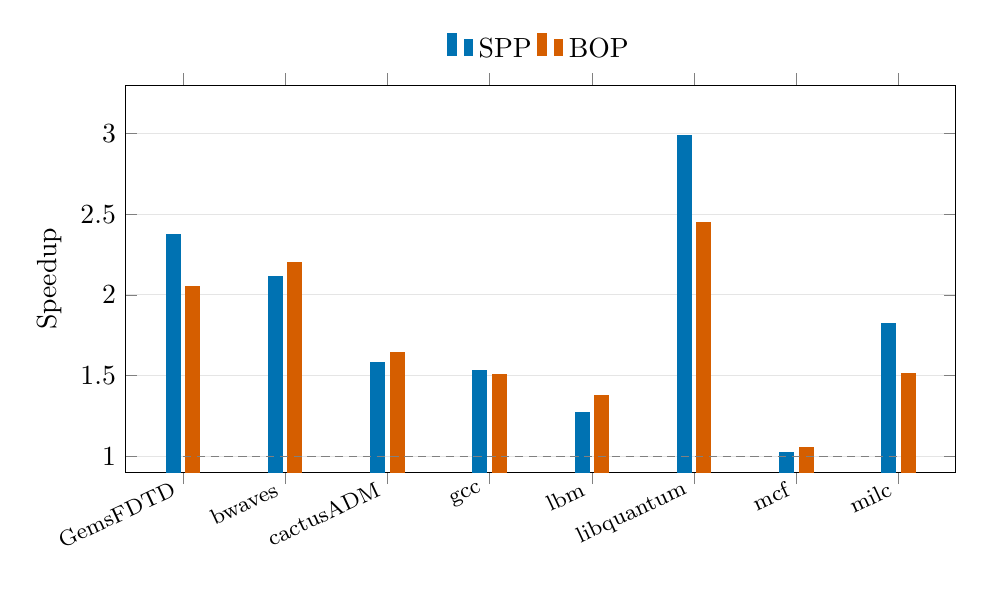
\begin{tikzpicture}
\begin{axis}[width=\linewidth,height=65mm,ybar,bar width=5pt,ymin=0.9,ymax=3.3,ylabel={Speedup},symbolic x coords={GemsFDTD,bwaves,cactusADM,gcc,lbm,libquantum,mcf,milc},xtick=data,x tick label style={rotate=25,anchor=east,font=\footnotesize},ytick={1,1.5,2,2.5,3},ymajorgrids,grid style={gray!20},legend style={at={(0.5,1.03)},anchor=south,legend columns=2,draw=none},enlarge x limits=0.08]
\addplot[fill=sppcolor,draw=sppcolor] coordinates {(GemsFDTD,2.3716)(bwaves,2.1131)(cactusADM,1.5800)(gcc,1.5307)(lbm,1.2679)(libquantum,2.9858)(mcf,1.0250)(milc,1.8239)};
\addplot[fill=bopcolor,draw=bopcolor] coordinates {(GemsFDTD,2.0489)(bwaves,2.2007)(cactusADM,1.6456)(gcc,1.5048)(lbm,1.3741)(libquantum,2.4492)(mcf,1.0554)(milc,1.5103)};
\legend{SPP,BOP}
\draw[densely dashed,gray] (axis cs:GemsFDTD,1) -- (axis cs:milc,1);
\end{axis}
\end{tikzpicture}
\caption{CPU2006 speedups from Table~\ref{tab:cpu2006}. Each bar is normalized to its application's no-prefetch run.}\label{fig:cpu2006}
\end{figure}
\FloatBarrier

The original single-core evaluation reports a 27.2\% average improvement over no L2 prefetching and a 6.4\% improvement over BOP\cite{kim2016}. It uses 18 memory-intensive CPU2006 applications with SimPoint sampling and three single-threaded CloudSuite workloads. Our eight-application reproduction gives a 74.45\% SPP improvement and an SPP/BOP geometric-mean ratio of approximately 1.0459. Both evaluations give SPP a higher average performance than BOP. The high speedups in libquantum and GemsFDTD contribute strongly to the mean in this reproduction.

\subsubsection{CPU2017 captured workloads}
The main result for each application combines the instruction and cycle counts from windows w1 and w2. Table~\ref{tab:cpu2017} reports IPC and speedup for the three configurations.

\begin{table}[htbp]
\centering\small
\caption{Primary CPU2017 results. Two windows per application, 200M warmup and 1B ROI per window.}\label{tab:cpu2017}
\begin{tabular}{@{}lrrrrr@{}}
\toprule
Application & No IPC & SPP IPC & SPP speedup & BOP IPC & BOP speedup\\
\midrule
bwaves & 0.374240 & 0.799424 & 2.1361 & 0.834683 & 2.2303\\
cactuBSSN & 0.770511 & 1.160332 & 1.5059 & 1.204875 & 1.5637\\
fotonik3d & 1.642059 & 1.642060 & 1.0000 & 1.642060 & 1.0000\\
lbm & 0.442673 & 0.549479 & 1.2413 & 0.599284 & 1.3538\\
mcf & 0.472226 & 0.539980 & 1.1435 & 0.522646 & 1.1068\\
omnetpp & 0.469010 & 0.468634 & 0.9992 & 0.468996 & 1.0000\\
xalancbmk & 0.340967 & 0.387294 & 1.1359 & 0.345593 & 1.0136\\
xz & 1.222644 & 1.234347 & 1.0096 & 1.240534 & 1.0146\\
\midrule
Geometric mean & & & \textbf{1.2298} & & \textbf{1.2339}\\
\bottomrule
\end{tabular}
\end{table}

The geometric mean speedups are 1.2298 for SPP and 1.2339 for BOP. SPP has the higher speedup in mcf and xalancbmk, while BOP has the higher speedup in bwaves, cactuBSSN, lbm, and xz. Fotonik3d and omnetpp remain close to their no-prefetch baselines.

Figure~\ref{fig:cpu2017} shows the application speedups in the same format as the CPU2006 comparison.
\begin{figure}[htbp]
\centering
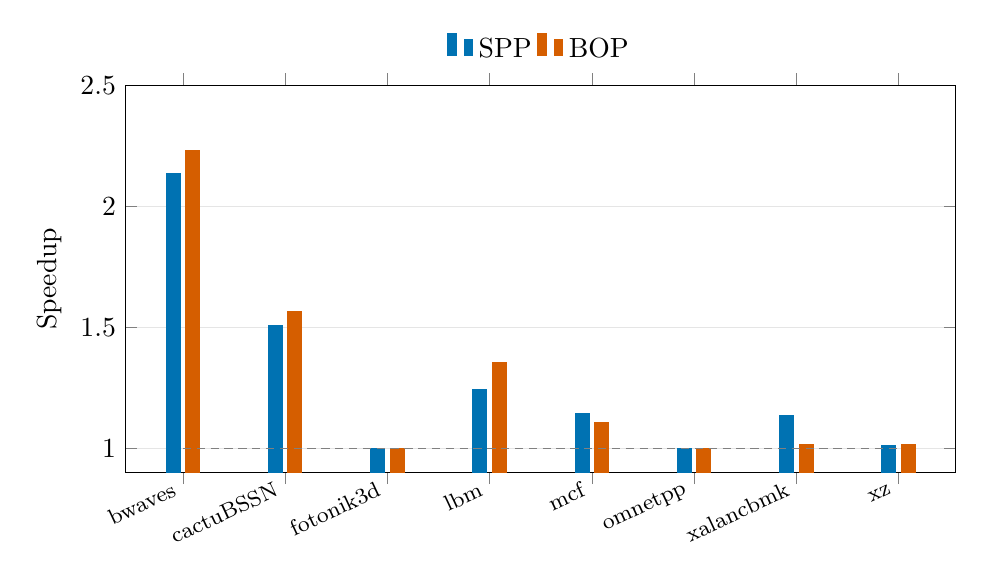
\begin{tikzpicture}
\begin{axis}[width=\linewidth,height=65mm,ybar,bar width=5pt,ymin=0.9,ymax=2.5,ylabel={Speedup},symbolic x coords={bwaves,cactuBSSN,fotonik3d,lbm,mcf,omnetpp,xalancbmk,xz},xtick=data,x tick label style={rotate=25,anchor=east,font=\footnotesize},ytick={1,1.5,2,2.5},ymajorgrids,grid style={gray!20},legend style={at={(0.5,1.03)},anchor=south,legend columns=2,draw=none},enlarge x limits=0.08]
\addplot[fill=sppcolor,draw=sppcolor] coordinates {(bwaves,2.1361)(cactuBSSN,1.5059)(fotonik3d,1.0000)(lbm,1.2413)(mcf,1.1435)(omnetpp,0.9992)(xalancbmk,1.1359)(xz,1.0096)};
\addplot[fill=bopcolor,draw=bopcolor] coordinates {(bwaves,2.2303)(cactuBSSN,1.5637)(fotonik3d,1.0000)(lbm,1.3538)(mcf,1.1068)(omnetpp,1.0000)(xalancbmk,1.0136)(xz,1.0146)};
\legend{SPP,BOP}
\draw[densely dashed,gray] (axis cs:bwaves,1) -- (axis cs:xz,1);
\end{axis}
\end{tikzpicture}
\caption{CPU2017 speedups from Table~\ref{tab:cpu2017}. Each bar is normalized to its application's no-prefetch result.}\label{fig:cpu2017}
\end{figure}
\FloatBarrier

\subsection{Lookahead and GHR component comparison}
The basic variant disables multistep lookahead and GHR. The lookahead variant enables path exploration, and full SPP also enables cross-page history.

\subsubsection{CPU2006 reproduction}
Table~\ref{tab:ablation} compares our component results with the values labelled in the original paper's component figure\cite{kim2016}.

\begin{table}[htbp]
\centering
\caption{Component speedups relative to each study's no-prefetch baseline.}\label{tab:ablation}
\begin{tabular}{@{}llrrr@{}}
\toprule
Source & Application or set & Basic & Lookahead & Full\\
\midrule
Original paper & Full workload set & 1.129 & 1.252 & 1.272\\
Original paper & libquantum & 1.118 & 1.332 & 1.349\\
This study & libquantum & 1.4122 & 2.9914 & 2.9858\\
Original paper & GemsFDTD & 1.140 & 1.399 & 1.444\\
This study & GemsFDTD & 2.0324 & 2.3586 & 2.3716\\
\bottomrule
\end{tabular}
\end{table}

Lookahead increases speedup in both measured applications. Libquantum increases from 1.4122 to 2.9914, while GemsFDTD increases from 2.0324 to 2.3586. This improvement agrees with the original paper's component results. Adding GHR gives a further increase in GemsFDTD and a small decrease in libquantum. The paper explains the usefulness of GHR in GemsFDTD through a recurring $(+30,+1)$ delta pattern that crosses a 4 KiB boundary, illustrating how GHR can preserve a pattern across pages.

In the paper, adding lookahead increases the performance improvement over the no-prefetch baseline by 21.4 percentage points for libquantum and 25.9 percentage points for GemsFDTD. GHR adds a further 4.5 percentage points for GemsFDTD. Our reproduction gives higher basic-SPP speedups and larger increases from lookahead. The paper also reports a mean lookahead depth of 6.9 across its traces.
\FloatBarrier

\subsubsection{CPU2017 captured workloads}
The CPU2017 component experiment compares basic, lookahead, and full SPP for bwaves and fotonik3d across both windows. These applications show contrasting responses in the main experiment: bwaves benefits substantially from SPP, while fotonik3d remains close to the baseline. The component comparison examines how lookahead and GHR contribute in each case. Table~\ref{tab:cpu2017ablation} reports the speedups aggregated across the two windows.
\begin{table}[htbp]
\centering
\caption{CPU2017 component speedups, combining w1 and w2.}\label{tab:cpu2017ablation}
\begin{tabular}{@{}lrrr@{}}
\toprule
Application & Basic & Lookahead & Full SPP\\
\midrule
bwaves & 1.6577 & 2.1390 & 2.1361\\
fotonik3d & 1.0000 & 1.0000 & 1.0000\\
\bottomrule
\end{tabular}
\end{table}
In bwaves, enabling lookahead raises speedup from 1.6577 to 2.1390. Full SPP gives 2.1361 after adding GHR. In fotonik3d, all three configurations give a speedup of 1.0000 at the displayed precision.

\subsection{Sensitivity to ROI length}
The CPU2006 ROI-length experiment keeps warmup at 200M instructions and compares measurement intervals of 500M and 1B instructions. Table~\ref{tab:window} shows that the relative ordering of SPP and BOP is unchanged for bwaves and mcf, although the speedup in bwaves changes with the measurement interval.
\begin{table}[htbp]
\centering
\caption{CPU2006 sensitivity to ROI length. Each interval has its matching baseline.}\label{tab:window}
\begin{tabular}{@{}lrrr@{}}
\toprule
Application & ROI instructions & SPP speedup & BOP speedup\\
\midrule
bwaves & 500M & 1.9682 & 2.1308\\
bwaves & 1B & 2.1131 & 2.2007\\
mcf & 500M & 1.0278 & 1.0605\\
mcf & 1B & 1.0250 & 1.0554\\
\bottomrule
\end{tabular}
\end{table}

\section{Additional Experiment: Confidence Threshold and Bandwidth}
The preceding experiments use a fixed prefetch confidence threshold. We expect this threshold and the available memory bandwidth to influence SPP performance together. A lower request threshold allows more predicted addresses to generate prefetch requests, potentially covering more future accesses while also increasing competition for memory service. A higher threshold selects candidates with greater confidence but can omit useful requests. The balance between these effects may change when memory bandwidth is reduced. This additional experiment therefore explores how SPP speedup responds to the request threshold under two bandwidth conditions.

We evaluate bwaves and mcf from both CPU2006 and CPU2017, using request thresholds of 15\%, 25\%, and 40\%. The normal and low bandwidth settings provide nominal bandwidths of 12.8 and 3.2 GB/s through channel widths of 8 and 2 bytes, respectively; other memory timing parameters remain unchanged. Each run uses 200M warmup instructions and a 1B-instruction ROI, with the CPU2017 experiment using window w1. The L2 fill threshold remains at 90\%, and the other SPP settings are held constant. Within each workload, all threshold settings use the same trace. Speedup is calculated against the no-prefetch configuration for the corresponding trace and bandwidth, allowing the threshold settings to be compared within each condition.

\begin{table}[htbp]
\centering\small
\caption{SPP speedup by request threshold and memory bandwidth for bwaves and mcf.}\label{tab:threshold}
\begin{tabular}{@{}lllrrr@{}}
\toprule
Benchmark & Application & Bandwidth & $T_P=15\%$ & $T_P=25\%$ & $T_P=40\%$\\
\midrule
CPU2006 & bwaves & Normal & 2.1051 & 2.1131 & 2.1181\\
 & & Low & 1.6126 & 1.6188 & 1.6345\\
 & mcf & Normal & 1.0344 & 1.0250 & 1.0123\\
 & & Low & 0.9904 & 0.9887 & 0.9866\\
\midrule
CPU2017 & bwaves & Normal & 2.2614 & 2.2669 & 2.2914\\
 & & Low & 1.6016 & 1.6083 & 1.6228\\
 & mcf & Normal & 1.2024 & 1.1956 & 1.1834\\
 & & Low & 1.1067 & 1.1205 & 1.1291\\
\bottomrule
\end{tabular}
\end{table}

Table~\ref{tab:threshold} shows that bwaves achieves its highest tested speedup at the 40\% request threshold in both benchmark versions and bandwidth conditions. Mcf favors 15\% under normal bandwidth in both versions; under low bandwidth, its highest tested speedup occurs at 15\% in CPU2006 and 40\% in CPU2017. The CPU2006 low-bandwidth mcf results remain below the no-prefetch baseline. The threshold that gives the best performance therefore depends on the application and bandwidth condition.

\section{Discussion and Conclusions}
SPP combines compressed delta history, conditional pattern learning, and multistep address prediction. Path confidence controls how far prediction proceeds, while filtering, fill targets, and cross-page history determine which requests are issued and where their data is placed. These mechanisms improve performance when useful data arrives in time to reduce demand-access stalls.

The CPU2006 reproduction obtains a geometric mean SPP speedup of 1.7445, compared with 1.6679 for BOP. The component comparison supports the benefit of lookahead in libquantum and GemsFDTD. Adding GHR gives a small increase in GemsFDTD and a small decrease in libquantum. Changing ROI length from 500M to 1B preserves the relative SPP/BOP ordering in bwaves and mcf, although the magnitude of the bwaves speedup changes.

For the captured CPU2017 windows, the geometric mean speedups are 1.2298 for SPP and 1.2339 for BOP. SPP performs better in mcf and xalancbmk, while BOP performs better in bwaves, cactuBSSN, lbm, and xz. Enabling lookahead in bwaves raises speedup from 1.6577 to 2.1390; in fotonik3d, all three component configurations remain at 1.0000 at the displayed precision.

Across the two evaluations, SPP's advantage over BOP in the CPU2006 set gives way to similar average performance in CPU2017. Both prefetchers also achieve smaller average gains over no prefetching in the CPU2017 set. The per-application results show how these averages arise: CPU2006 includes large SPP gains in GemsFDTD, libquantum, and bwaves, whereas CPU2017 includes several applications close to the no-prefetch baseline, such as fotonik3d, omnetpp, and xz. Among applications present in both sets, bwaves retains a substantial benefit and mcf shows a larger SPP benefit in the CPU2017 samples. The overall results therefore depend on the distribution of gains across the selected applications and execution windows.

The component experiments also connect the original evaluation with the CPU2017 extension. The original paper and the CPU2006 reproduction both show benefits from lookahead in libquantum and GemsFDTD; the CPU2017 bwaves result shows that this benefit also occurs in the newer workload set. GHR has a less consistent effect: it improves GemsFDTD in the reproduction, slightly reduces speedup in CPU2017 bwaves, and produces no visible change in fotonik3d at the reported precision. These comparisons show that lookahead can provide substantial gains, while the additional contribution of cross-page history varies with the application. The threshold experiment further shows that the best tested setting can change with bandwidth, as observed for CPU2017 mcf.

Future work could examine the effect of warmup length. Warmup establishes cache contents and trains the signature and pattern tables before measurement begins. Varying its length while keeping the measured instruction window fixed would help determine how quickly SPP reaches stable performance and whether different applications require different training lengths. The comparison could track speedup and prefetch accuracy across several warmup settings, providing a basis for selecting the warmup length in subsequent experiments.

Another direction is to compare SPP operating at L1, L2, and LLC. The current implementation operates at L2 and selects L2 or LLC as the destination for its requests. Moving the predictor to a different cache level would change the access stream used for training and the time available for predictions to become useful. A follow-up experiment could implement SPP at each level with comparable prediction-table storage, specify the accesses used for training and the destination of requests, and compare speedup, useful prefetches, and memory traffic. This would help identify which placement suits each application's access pattern and how confidence thresholds should be chosen for that placement.

\appendix
\section{Experimental Configuration}\label{app:configuration}
\subsection{Processor and memory parameters}
Table~\ref{tab:hardware} lists the hardware model. The low-bandwidth condition in the additional experiment uses a 2-byte channel width (3.2 GB/s nominal), with other timing parameters unchanged.
\begin{table}[htbp]
\centering
\caption{Processor, cache, and memory configuration.}\label{tab:hardware}
\begin{tabularx}{\linewidth}{@{}p{33mm}Y@{}}
\toprule
Component & Configuration\\
\midrule
Core & Single out-of-order core, 3.2 GHz, 4-wide fetch/decode/dispatch/execute/retire, ROB 256, LQ/SQ 64 each\\
Branch prediction & Gshare, basic\_btb, 20-cycle misprediction penalty\\
L1I and L1D & 32 KiB each, 8-way, 4-cycle latency, 8 MSHRs each\\
L2 & 256 KiB, 8-way, 8-cycle latency, 16 MSHRs, prefetch queue 16\\
LLC & 2 MiB, 16-way, 12-cycle latency, 32 MSHRs, prefetch queue 32\\
Address units & 64-byte cache line, 4 KiB page\\
DRAM & 1 channel, 1600 MT/s, 2 ranks, 8 banks; tCAS/tRCD/tRP 24 and tRAS 52 memory-controller cycles\\
Memory bandwidth & Channel width 8 bytes (12.8 GB/s nominal)\\
SPP thresholds & Request threshold $T_P=0.25$, L2 fill threshold $T_F=0.90$\\
Measurement & 200M warmup instructions, 1B ROI instructions for primary comparisons\\
\bottomrule
\end{tabularx}
\end{table}

\subsection{Prefetcher settings}
BOP follows best-offset learning\cite{michaud2016}. It uses 46 signed candidate offsets, two recent-request tables of 64 entries each, and a 15-entry delay queue with a delay of 60 simulated cycles. Learning stops after 100 rounds or a score of 31. Request generation respects page boundaries and includes the mechanism's MSHR and LLC throttling. BOP retains LOAD, RFO, and PREFETCH activation; SPP uses LOAD and PREFETCH activation and its internal training rules.

\subsection{CPU2017 inputs and capture settings}
The programs are built on Linux x86-64 with GCC, G++, and GFortran.

The base options are \code{-O2}, \code{-fno-tree-vectorize}, and \code{-m64}, with the required SPEC portability options. Each application uses one copy and the first command in its \code{specinvoke} ref command list. Table~\ref{tab:workloads} lists the selected inputs.

\begin{table}[htbp]
\centering\small
\caption{Primary SPEC CPU2017 applications and selected ref inputs.}\label{tab:workloads}
\begin{tabularx}{\linewidth}{@{}p{26mm}p{37mm}Y@{}}
\toprule
Application & SPEC program & Input or selected call\\
\midrule
bwaves & \code{503.bwaves\_r} & First call, stdin \code{bwaves\_1.in}\\
cactuBSSN & \code{507.cactuBSSN\_r} & \code{spec\_ref.par}\\
fotonik3d & \code{549.fotonik3d\_r} & Ref optical input files, including \code{OBJ.dat} and \code{PSI.dat}\\
lbm & \code{519.lbm\_r} & \code{3000 reference.dat 0 0}, \code{100\_100\_130\_ldc.of}\\
mcf & \code{505.mcf\_r} & \code{inp.in}\\
omnetpp & \code{520.omnetpp\_r} & \code{-c General -r 0}, \code{omnetpp.ini} and NED files\\
xalancbmk & \code{523.xalancbmk\_r} & \code{-v t5.xml xalanc.xsl}\\
xz & \code{557.xz\_r} & First call, \code{cld.tar.xz}, 160 MiB input, compression level 6\\
\bottomrule
\end{tabularx}
\end{table}
Window w1 skips 1 billion dynamic instructions before capture; w2 skips 10 billion. Each trace contains 1.21 billion records, including a margin beyond the 200M warmup and 1B ROI.

\subsection{File locations}
Table~\ref{tab:files} gives paths relative to the project root.

The prefix \code{stage/} in the table denotes \code{work/cpu2017\_delivery\_20261005/}.

\begin{table}[htbp]
\centering\small
\caption{Source, configuration, and result file locations.}\label{tab:files}
\begin{tabularx}{\linewidth}{@{}p{43mm}Y@{}}
\toprule
File & Location relative to the project root\\
\midrule
SPP implementation & \code{patches/spp\_dev/spp\_dev.cc}\\
BOP implementation & \code{patches/bop/bop.cc}\\
Processor configuration & \code{configs/paper\_base.json}\\
Full SPP configuration & \code{configs/spp\_full.json}\\
SPEC compilation configuration & \code{configs/spec\_cpu2017\_gcc11\_O2.cfg}\\
Simulation entry & \code{scripts/run\_experiment.py}\\
CPU2017 capture script & \code{stage/capture\_cpu2017\_self\_v2.py}\\
Formal simulation results & \code{stage/delivery\_results/formal\_all.csv}\\
Application performance & \code{stage/delivery\_results/application\_metrics.csv}\\
Component comparison & \code{stage/report\_metrics/ablation\_metrics.csv}\\
Threshold comparison & \code{stage/report\_metrics/threshold\_metrics.csv}\\
\bottomrule
\end{tabularx}
\end{table}

\section{AI Use Statement}\label{app:tools}
Codex assisted with implementation and debugging, organizing experiments, writing analysis scripts, and preparing the report. This included suggesting code changes, processing experimental outputs, and revising the report's wording and structure. Code changes were checked by running the code, and the reported numerical results were checked against the recorded experimental outputs. The analysis and conclusions are based on those results.

\begin{thebibliography}{9}
\bibitem{kim2016} Jinchun Kim, Seth H. Pugsley, Paul V. Gratz, A. L. Narasimha Reddy, Chris Wilkerson, and Zeshan Chishti. \textit{Path Confidence Based Lookahead Prefetching}. IEEE/ACM International Symposium on Microarchitecture (MICRO), 2016. \href{https://doi.org/10.1109/MICRO.2016.7783763}{doi:10.1109/MICRO.2016.7783763}.
\bibitem{michaud2016} Pierre Michaud. \textit{Best-Offset Hardware Prefetching}. IEEE International Symposium on High Performance Computer Architecture (HPCA), 2016. \href{https://doi.org/10.1109/HPCA.2016.7446087}{doi:10.1109/HPCA.2016.7446087}.
\bibitem{champsim} ChampSim Project. \textit{ChampSim source and documentation}. \url{https://github.com/ChampSim/ChampSim}.
\bibitem{spec2017} Standard Performance Evaluation Corporation. \textit{SPEC CPU2017}. \url{https://www.spec.org/cpu2017/}.
\bibitem{pin} Intel. \textit{Pin: A Dynamic Binary Instrumentation Tool}. \url{https://www.intel.com/content/www/us/en/developer/articles/tool/pin-a-dynamic-binary-instrumentation-tool.html}.
\bibitem{trace2006} Dimitrios Chasapis. \textit{SPEC CPU 2006 ChampSim Traces}. Zenodo, 2024, record 10959705. \href{https://doi.org/10.5281/zenodo.10959705}{doi:10.5281/zenodo.10959705}.
\end{thebibliography}
\end{document}
